% Created by tikzDevice version 0.12.3.1 on 2022-05-26 15:24:44
% !TEX encoding = UTF-8 Unicode
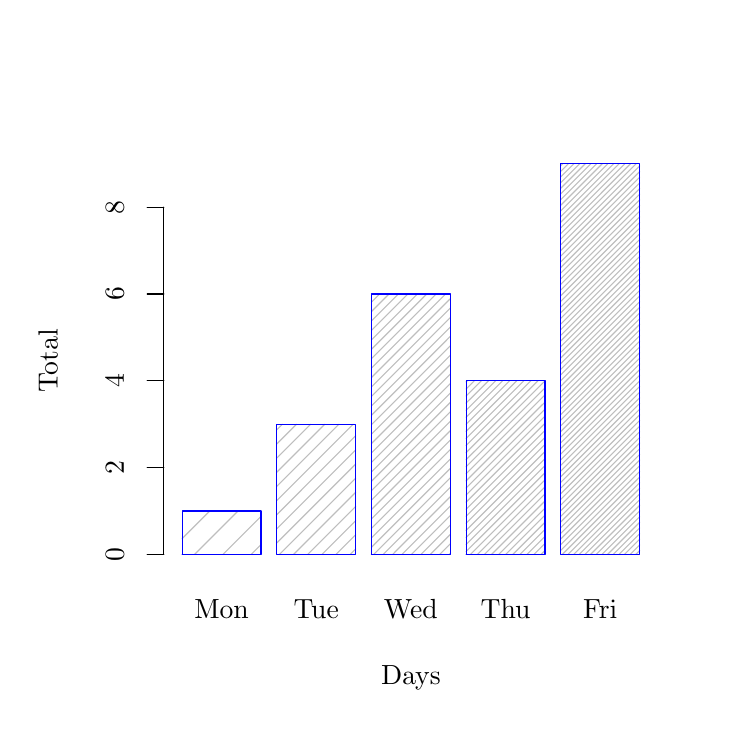
\begin{tikzpicture}[x=1pt,y=1pt]
\definecolor{fillColor}{RGB}{255,255,255}
\path[use as bounding box,fill=fillColor,fill opacity=0.00] (0,0) rectangle (252.94,252.94);
\begin{scope}
\path[clip] (  0.00,  0.00) rectangle (252.94,252.94);
\definecolor{drawColor}{RGB}{190,190,190}

\path[draw=drawColor,line width= 0.4pt,line join=round,line cap=round] ( 55.81, 68.31) -- ( 65.79, 78.29);

\path[draw=drawColor,line width= 0.4pt,line join=round,line cap=round] ( 60.33, 62.61) -- ( 76.01, 78.29);

\path[draw=drawColor,line width= 0.4pt,line join=round,line cap=round] ( 70.55, 62.61) -- ( 84.32, 76.37);

\path[draw=drawColor,line width= 0.4pt,line join=round,line cap=round] ( 80.77, 62.61) -- ( 84.32, 66.15);

\path[draw=drawColor,line width= 0.4pt,line join=round,line cap=round] ( 90.02,107.63) -- ( 92.05,109.66);

\path[draw=drawColor,line width= 0.4pt,line join=round,line cap=round] ( 90.02,102.52) -- ( 97.16,109.66);

\path[draw=drawColor,line width= 0.4pt,line join=round,line cap=round] ( 90.02, 97.41) -- (102.27,109.66);

\path[draw=drawColor,line width= 0.4pt,line join=round,line cap=round] ( 90.02, 92.30) -- (107.38,109.66);

\path[draw=drawColor,line width= 0.4pt,line join=round,line cap=round] ( 90.02, 87.19) -- (112.49,109.66);

\path[draw=drawColor,line width= 0.4pt,line join=round,line cap=round] ( 90.02, 82.07) -- (117.60,109.66);

\path[draw=drawColor,line width= 0.4pt,line join=round,line cap=round] ( 90.02, 76.96) -- (118.52,105.47);

\path[draw=drawColor,line width= 0.4pt,line join=round,line cap=round] ( 90.02, 71.85) -- (118.52,100.36);

\path[draw=drawColor,line width= 0.4pt,line join=round,line cap=round] ( 90.02, 66.74) -- (118.52, 95.25);

\path[draw=drawColor,line width= 0.4pt,line join=round,line cap=round] ( 90.99, 62.61) -- (118.52, 90.14);

\path[draw=drawColor,line width= 0.4pt,line join=round,line cap=round] ( 96.10, 62.61) -- (118.52, 85.03);

\path[draw=drawColor,line width= 0.4pt,line join=round,line cap=round] (101.21, 62.61) -- (118.52, 79.92);

\path[draw=drawColor,line width= 0.4pt,line join=round,line cap=round] (106.32, 62.61) -- (118.52, 74.81);

\path[draw=drawColor,line width= 0.4pt,line join=round,line cap=round] (111.44, 62.61) -- (118.52, 69.70);

\path[draw=drawColor,line width= 0.4pt,line join=round,line cap=round] (116.55, 62.61) -- (118.52, 64.59);

\path[draw=drawColor,line width= 0.4pt,line join=round,line cap=round] (124.22,153.75) -- (127.17,156.70);

\path[draw=drawColor,line width= 0.4pt,line join=round,line cap=round] (124.22,150.35) -- (130.57,156.70);

\path[draw=drawColor,line width= 0.4pt,line join=round,line cap=round] (124.22,146.94) -- (133.98,156.70);

\path[draw=drawColor,line width= 0.4pt,line join=round,line cap=round] (124.22,143.53) -- (137.39,156.70);

\path[draw=drawColor,line width= 0.4pt,line join=round,line cap=round] (124.22,140.13) -- (140.79,156.70);

\path[draw=drawColor,line width= 0.4pt,line join=round,line cap=round] (124.22,136.72) -- (144.20,156.70);

\path[draw=drawColor,line width= 0.4pt,line join=round,line cap=round] (124.22,133.31) -- (147.61,156.70);

\path[draw=drawColor,line width= 0.4pt,line join=round,line cap=round] (124.22,129.91) -- (151.01,156.70);

\path[draw=drawColor,line width= 0.4pt,line join=round,line cap=round] (124.22,126.50) -- (152.72,155.00);

\path[draw=drawColor,line width= 0.4pt,line join=round,line cap=round] (124.22,123.09) -- (152.72,151.60);

\path[draw=drawColor,line width= 0.4pt,line join=round,line cap=round] (124.22,119.69) -- (152.72,148.19);

\path[draw=drawColor,line width= 0.4pt,line join=round,line cap=round] (124.22,116.28) -- (152.72,144.78);

\path[draw=drawColor,line width= 0.4pt,line join=round,line cap=round] (124.22,112.87) -- (152.72,141.38);

\path[draw=drawColor,line width= 0.4pt,line join=round,line cap=round] (124.22,109.47) -- (152.72,137.97);

\path[draw=drawColor,line width= 0.4pt,line join=round,line cap=round] (124.22,106.06) -- (152.72,134.56);

\path[draw=drawColor,line width= 0.4pt,line join=round,line cap=round] (124.22,102.65) -- (152.72,131.16);

\path[draw=drawColor,line width= 0.4pt,line join=round,line cap=round] (124.22, 99.24) -- (152.72,127.75);

\path[draw=drawColor,line width= 0.4pt,line join=round,line cap=round] (124.22, 95.84) -- (152.72,124.34);

\path[draw=drawColor,line width= 0.4pt,line join=round,line cap=round] (124.22, 92.43) -- (152.72,120.93);

\path[draw=drawColor,line width= 0.4pt,line join=round,line cap=round] (124.22, 89.02) -- (152.72,117.53);

\path[draw=drawColor,line width= 0.4pt,line join=round,line cap=round] (124.22, 85.62) -- (152.72,114.12);

\path[draw=drawColor,line width= 0.4pt,line join=round,line cap=round] (124.22, 82.21) -- (152.72,110.71);

\path[draw=drawColor,line width= 0.4pt,line join=round,line cap=round] (124.22, 78.80) -- (152.72,107.31);

\path[draw=drawColor,line width= 0.4pt,line join=round,line cap=round] (124.22, 75.40) -- (152.72,103.90);

\path[draw=drawColor,line width= 0.4pt,line join=round,line cap=round] (124.22, 71.99) -- (152.72,100.49);

\path[draw=drawColor,line width= 0.4pt,line join=round,line cap=round] (124.22, 68.58) -- (152.72, 97.09);

\path[draw=drawColor,line width= 0.4pt,line join=round,line cap=round] (124.22, 65.18) -- (152.72, 93.68);

\path[draw=drawColor,line width= 0.4pt,line join=round,line cap=round] (125.06, 62.61) -- (152.72, 90.27);

\path[draw=drawColor,line width= 0.4pt,line join=round,line cap=round] (128.47, 62.61) -- (152.72, 86.87);

\path[draw=drawColor,line width= 0.4pt,line join=round,line cap=round] (131.88, 62.61) -- (152.72, 83.46);

\path[draw=drawColor,line width= 0.4pt,line join=round,line cap=round] (135.28, 62.61) -- (152.72, 80.05);

\path[draw=drawColor,line width= 0.4pt,line join=round,line cap=round] (138.69, 62.61) -- (152.72, 76.65);

\path[draw=drawColor,line width= 0.4pt,line join=round,line cap=round] (142.10, 62.61) -- (152.72, 73.24);

\path[draw=drawColor,line width= 0.4pt,line join=round,line cap=round] (145.50, 62.61) -- (152.72, 69.83);

\path[draw=drawColor,line width= 0.4pt,line join=round,line cap=round] (148.91, 62.61) -- (152.72, 66.43);

\path[draw=drawColor,line width= 0.4pt,line join=round,line cap=round] (152.32, 62.61) -- (152.72, 63.02);

\path[draw=drawColor,line width= 0.4pt,line join=round,line cap=round] (158.42,124.93) -- (158.83,125.34);

\path[draw=drawColor,line width= 0.4pt,line join=round,line cap=round] (158.42,122.38) -- (161.39,125.34);

\path[draw=drawColor,line width= 0.4pt,line join=round,line cap=round] (158.42,119.82) -- (163.94,125.34);

\path[draw=drawColor,line width= 0.4pt,line join=round,line cap=round] (158.42,117.27) -- (166.50,125.34);

\path[draw=drawColor,line width= 0.4pt,line join=round,line cap=round] (158.42,114.71) -- (169.05,125.34);

\path[draw=drawColor,line width= 0.4pt,line join=round,line cap=round] (158.42,112.16) -- (171.61,125.34);

\path[draw=drawColor,line width= 0.4pt,line join=round,line cap=round] (158.42,109.60) -- (174.16,125.34);

\path[draw=drawColor,line width= 0.4pt,line join=round,line cap=round] (158.42,107.05) -- (176.72,125.34);

\path[draw=drawColor,line width= 0.4pt,line join=round,line cap=round] (158.42,104.49) -- (179.27,125.34);

\path[draw=drawColor,line width= 0.4pt,line join=round,line cap=round] (158.42,101.94) -- (181.83,125.34);

\path[draw=drawColor,line width= 0.4pt,line join=round,line cap=round] (158.42, 99.38) -- (184.38,125.34);

\path[draw=drawColor,line width= 0.4pt,line join=round,line cap=round] (158.42, 96.83) -- (186.93,125.33);

\path[draw=drawColor,line width= 0.4pt,line join=round,line cap=round] (158.42, 94.27) -- (186.93,122.77);

\path[draw=drawColor,line width= 0.4pt,line join=round,line cap=round] (158.42, 91.72) -- (186.93,120.22);

\path[draw=drawColor,line width= 0.4pt,line join=round,line cap=round] (158.42, 89.16) -- (186.93,117.66);

\path[draw=drawColor,line width= 0.4pt,line join=round,line cap=round] (158.42, 86.60) -- (186.93,115.11);

\path[draw=drawColor,line width= 0.4pt,line join=round,line cap=round] (158.42, 84.05) -- (186.93,112.55);

\path[draw=drawColor,line width= 0.4pt,line join=round,line cap=round] (158.42, 81.49) -- (186.93,110.00);

\path[draw=drawColor,line width= 0.4pt,line join=round,line cap=round] (158.42, 78.94) -- (186.93,107.44);

\path[draw=drawColor,line width= 0.4pt,line join=round,line cap=round] (158.42, 76.38) -- (186.93,104.89);

\path[draw=drawColor,line width= 0.4pt,line join=round,line cap=round] (158.42, 73.83) -- (186.93,102.33);

\path[draw=drawColor,line width= 0.4pt,line join=round,line cap=round] (158.42, 71.27) -- (186.93, 99.78);

\path[draw=drawColor,line width= 0.4pt,line join=round,line cap=round] (158.42, 68.72) -- (186.93, 97.22);

\path[draw=drawColor,line width= 0.4pt,line join=round,line cap=round] (158.42, 66.16) -- (186.93, 94.67);

\path[draw=drawColor,line width= 0.4pt,line join=round,line cap=round] (158.42, 63.61) -- (186.93, 92.11);

\path[draw=drawColor,line width= 0.4pt,line join=round,line cap=round] (159.98, 62.61) -- (186.93, 89.56);

\path[draw=drawColor,line width= 0.4pt,line join=round,line cap=round] (162.54, 62.61) -- (186.93, 87.00);

\path[draw=drawColor,line width= 0.4pt,line join=round,line cap=round] (165.09, 62.61) -- (186.93, 84.45);

\path[draw=drawColor,line width= 0.4pt,line join=round,line cap=round] (167.65, 62.61) -- (186.93, 81.89);

\path[draw=drawColor,line width= 0.4pt,line join=round,line cap=round] (170.20, 62.61) -- (186.93, 79.34);

\path[draw=drawColor,line width= 0.4pt,line join=round,line cap=round] (172.76, 62.61) -- (186.93, 76.78);

\path[draw=drawColor,line width= 0.4pt,line join=round,line cap=round] (175.31, 62.61) -- (186.93, 74.23);

\path[draw=drawColor,line width= 0.4pt,line join=round,line cap=round] (177.87, 62.61) -- (186.93, 71.67);

\path[draw=drawColor,line width= 0.4pt,line join=round,line cap=round] (180.42, 62.61) -- (186.93, 69.12);

\path[draw=drawColor,line width= 0.4pt,line join=round,line cap=round] (182.98, 62.61) -- (186.93, 66.56);

\path[draw=drawColor,line width= 0.4pt,line join=round,line cap=round] (185.53, 62.61) -- (186.93, 64.01);

\path[draw=drawColor,line width= 0.4pt,line join=round,line cap=round] (192.63,203.08) -- (193.29,203.75);

\path[draw=drawColor,line width= 0.4pt,line join=round,line cap=round] (192.63,201.04) -- (195.33,203.75);

\path[draw=drawColor,line width= 0.4pt,line join=round,line cap=round] (192.63,199.00) -- (197.38,203.75);

\path[draw=drawColor,line width= 0.4pt,line join=round,line cap=round] (192.63,196.95) -- (199.42,203.75);

\path[draw=drawColor,line width= 0.4pt,line join=round,line cap=round] (192.63,194.91) -- (201.47,203.75);

\path[draw=drawColor,line width= 0.4pt,line join=round,line cap=round] (192.63,192.86) -- (203.51,203.75);

\path[draw=drawColor,line width= 0.4pt,line join=round,line cap=round] (192.63,190.82) -- (205.55,203.75);

\path[draw=drawColor,line width= 0.4pt,line join=round,line cap=round] (192.63,188.78) -- (207.60,203.75);

\path[draw=drawColor,line width= 0.4pt,line join=round,line cap=round] (192.63,186.73) -- (209.64,203.75);

\path[draw=drawColor,line width= 0.4pt,line join=round,line cap=round] (192.63,184.69) -- (211.69,203.75);

\path[draw=drawColor,line width= 0.4pt,line join=round,line cap=round] (192.63,182.64) -- (213.73,203.75);

\path[draw=drawColor,line width= 0.4pt,line join=round,line cap=round] (192.63,180.60) -- (215.78,203.75);

\path[draw=drawColor,line width= 0.4pt,line join=round,line cap=round] (192.63,178.55) -- (217.82,203.75);

\path[draw=drawColor,line width= 0.4pt,line join=round,line cap=round] (192.63,176.51) -- (219.86,203.75);

\path[draw=drawColor,line width= 0.4pt,line join=round,line cap=round] (192.63,174.47) -- (221.13,202.97);

\path[draw=drawColor,line width= 0.4pt,line join=round,line cap=round] (192.63,172.42) -- (221.13,200.93);

\path[draw=drawColor,line width= 0.4pt,line join=round,line cap=round] (192.63,170.38) -- (221.13,198.88);

\path[draw=drawColor,line width= 0.4pt,line join=round,line cap=round] (192.63,168.33) -- (221.13,196.84);

\path[draw=drawColor,line width= 0.4pt,line join=round,line cap=round] (192.63,166.29) -- (221.13,194.79);

\path[draw=drawColor,line width= 0.4pt,line join=round,line cap=round] (192.63,164.25) -- (221.13,192.75);

\path[draw=drawColor,line width= 0.4pt,line join=round,line cap=round] (192.63,162.20) -- (221.13,190.71);

\path[draw=drawColor,line width= 0.4pt,line join=round,line cap=round] (192.63,160.16) -- (221.13,188.66);

\path[draw=drawColor,line width= 0.4pt,line join=round,line cap=round] (192.63,158.11) -- (221.13,186.62);

\path[draw=drawColor,line width= 0.4pt,line join=round,line cap=round] (192.63,156.07) -- (221.13,184.57);

\path[draw=drawColor,line width= 0.4pt,line join=round,line cap=round] (192.63,154.03) -- (221.13,182.53);

\path[draw=drawColor,line width= 0.4pt,line join=round,line cap=round] (192.63,151.98) -- (221.13,180.48);

\path[draw=drawColor,line width= 0.4pt,line join=round,line cap=round] (192.63,149.94) -- (221.13,178.44);

\path[draw=drawColor,line width= 0.4pt,line join=round,line cap=round] (192.63,147.89) -- (221.13,176.40);

\path[draw=drawColor,line width= 0.4pt,line join=round,line cap=round] (192.63,145.85) -- (221.13,174.35);

\path[draw=drawColor,line width= 0.4pt,line join=round,line cap=round] (192.63,143.80) -- (221.13,172.31);

\path[draw=drawColor,line width= 0.4pt,line join=round,line cap=round] (192.63,141.76) -- (221.13,170.26);

\path[draw=drawColor,line width= 0.4pt,line join=round,line cap=round] (192.63,139.72) -- (221.13,168.22);

\path[draw=drawColor,line width= 0.4pt,line join=round,line cap=round] (192.63,137.67) -- (221.13,166.18);

\path[draw=drawColor,line width= 0.4pt,line join=round,line cap=round] (192.63,135.63) -- (221.13,164.13);

\path[draw=drawColor,line width= 0.4pt,line join=round,line cap=round] (192.63,133.58) -- (221.13,162.09);

\path[draw=drawColor,line width= 0.4pt,line join=round,line cap=round] (192.63,131.54) -- (221.13,160.04);

\path[draw=drawColor,line width= 0.4pt,line join=round,line cap=round] (192.63,129.50) -- (221.13,158.00);

\path[draw=drawColor,line width= 0.4pt,line join=round,line cap=round] (192.63,127.45) -- (221.13,155.96);

\path[draw=drawColor,line width= 0.4pt,line join=round,line cap=round] (192.63,125.41) -- (221.13,153.91);

\path[draw=drawColor,line width= 0.4pt,line join=round,line cap=round] (192.63,123.36) -- (221.13,151.87);

\path[draw=drawColor,line width= 0.4pt,line join=round,line cap=round] (192.63,121.32) -- (221.13,149.82);

\path[draw=drawColor,line width= 0.4pt,line join=round,line cap=round] (192.63,119.28) -- (221.13,147.78);

\path[draw=drawColor,line width= 0.4pt,line join=round,line cap=round] (192.63,117.23) -- (221.13,145.73);

\path[draw=drawColor,line width= 0.4pt,line join=round,line cap=round] (192.63,115.19) -- (221.13,143.69);

\path[draw=drawColor,line width= 0.4pt,line join=round,line cap=round] (192.63,113.14) -- (221.13,141.65);

\path[draw=drawColor,line width= 0.4pt,line join=round,line cap=round] (192.63,111.10) -- (221.13,139.60);

\path[draw=drawColor,line width= 0.4pt,line join=round,line cap=round] (192.63,109.06) -- (221.13,137.56);

\path[draw=drawColor,line width= 0.4pt,line join=round,line cap=round] (192.63,107.01) -- (221.13,135.51);

\path[draw=drawColor,line width= 0.4pt,line join=round,line cap=round] (192.63,104.97) -- (221.13,133.47);

\path[draw=drawColor,line width= 0.4pt,line join=round,line cap=round] (192.63,102.92) -- (221.13,131.43);

\path[draw=drawColor,line width= 0.4pt,line join=round,line cap=round] (192.63,100.88) -- (221.13,129.38);

\path[draw=drawColor,line width= 0.4pt,line join=round,line cap=round] (192.63, 98.83) -- (221.13,127.34);

\path[draw=drawColor,line width= 0.4pt,line join=round,line cap=round] (192.63, 96.79) -- (221.13,125.29);

\path[draw=drawColor,line width= 0.4pt,line join=round,line cap=round] (192.63, 94.75) -- (221.13,123.25);

\path[draw=drawColor,line width= 0.4pt,line join=round,line cap=round] (192.63, 92.70) -- (221.13,121.21);

\path[draw=drawColor,line width= 0.4pt,line join=round,line cap=round] (192.63, 90.66) -- (221.13,119.16);

\path[draw=drawColor,line width= 0.4pt,line join=round,line cap=round] (192.63, 88.61) -- (221.13,117.12);

\path[draw=drawColor,line width= 0.4pt,line join=round,line cap=round] (192.63, 86.57) -- (221.13,115.07);

\path[draw=drawColor,line width= 0.4pt,line join=round,line cap=round] (192.63, 84.53) -- (221.13,113.03);

\path[draw=drawColor,line width= 0.4pt,line join=round,line cap=round] (192.63, 82.48) -- (221.13,110.99);

\path[draw=drawColor,line width= 0.4pt,line join=round,line cap=round] (192.63, 80.44) -- (221.13,108.94);

\path[draw=drawColor,line width= 0.4pt,line join=round,line cap=round] (192.63, 78.39) -- (221.13,106.90);

\path[draw=drawColor,line width= 0.4pt,line join=round,line cap=round] (192.63, 76.35) -- (221.13,104.85);

\path[draw=drawColor,line width= 0.4pt,line join=round,line cap=round] (192.63, 74.31) -- (221.13,102.81);

\path[draw=drawColor,line width= 0.4pt,line join=round,line cap=round] (192.63, 72.26) -- (221.13,100.76);

\path[draw=drawColor,line width= 0.4pt,line join=round,line cap=round] (192.63, 70.22) -- (221.13, 98.72);

\path[draw=drawColor,line width= 0.4pt,line join=round,line cap=round] (192.63, 68.17) -- (221.13, 96.68);

\path[draw=drawColor,line width= 0.4pt,line join=round,line cap=round] (192.63, 66.13) -- (221.13, 94.63);

\path[draw=drawColor,line width= 0.4pt,line join=round,line cap=round] (192.63, 64.08) -- (221.13, 92.59);

\path[draw=drawColor,line width= 0.4pt,line join=round,line cap=round] (193.20, 62.61) -- (221.13, 90.54);

\path[draw=drawColor,line width= 0.4pt,line join=round,line cap=round] (195.24, 62.61) -- (221.13, 88.50);

\path[draw=drawColor,line width= 0.4pt,line join=round,line cap=round] (197.29, 62.61) -- (221.13, 86.46);

\path[draw=drawColor,line width= 0.4pt,line join=round,line cap=round] (199.33, 62.61) -- (221.13, 84.41);

\path[draw=drawColor,line width= 0.4pt,line join=round,line cap=round] (201.38, 62.61) -- (221.13, 82.37);

\path[draw=drawColor,line width= 0.4pt,line join=round,line cap=round] (203.42, 62.61) -- (221.13, 80.32);

\path[draw=drawColor,line width= 0.4pt,line join=round,line cap=round] (205.46, 62.61) -- (221.13, 78.28);

\path[draw=drawColor,line width= 0.4pt,line join=round,line cap=round] (207.51, 62.61) -- (221.13, 76.24);

\path[draw=drawColor,line width= 0.4pt,line join=round,line cap=round] (209.55, 62.61) -- (221.13, 74.19);

\path[draw=drawColor,line width= 0.4pt,line join=round,line cap=round] (211.60, 62.61) -- (221.13, 72.15);

\path[draw=drawColor,line width= 0.4pt,line join=round,line cap=round] (213.64, 62.61) -- (221.13, 70.10);

\path[draw=drawColor,line width= 0.4pt,line join=round,line cap=round] (215.68, 62.61) -- (221.13, 68.06);

\path[draw=drawColor,line width= 0.4pt,line join=round,line cap=round] (217.73, 62.61) -- (221.13, 66.01);

\path[draw=drawColor,line width= 0.4pt,line join=round,line cap=round] (219.77, 62.61) -- (221.13, 63.97);
\definecolor{drawColor}{RGB}{0,0,255}

\path[draw=drawColor,line width= 0.4pt,line join=round,line cap=round] ( 55.81, 62.61) --
	( 84.32, 62.61) --
	( 84.32, 78.29) --
	( 55.81, 78.29) --
	( 55.81, 62.61);

\path[draw=drawColor,line width= 0.4pt,line join=round,line cap=round] ( 90.02, 62.61) --
	(118.52, 62.61) --
	(118.52,109.66) --
	( 90.02,109.66) --
	( 90.02, 62.61);

\path[draw=drawColor,line width= 0.4pt,line join=round,line cap=round] (124.22, 62.61) --
	(152.72, 62.61) --
	(152.72,156.70) --
	(124.22,156.70) --
	(124.22, 62.61);

\path[draw=drawColor,line width= 0.4pt,line join=round,line cap=round] (158.42, 62.61) --
	(186.93, 62.61) --
	(186.93,125.34) --
	(158.42,125.34) --
	(158.42, 62.61);

\path[draw=drawColor,line width= 0.4pt,line join=round,line cap=round] (192.63, 62.61) --
	(221.13, 62.61) --
	(221.13,203.75) --
	(192.63,203.75) --
	(192.63, 62.61);
\end{scope}
\begin{scope}
\path[clip] (  0.00,  0.00) rectangle (252.94,252.94);
\definecolor{drawColor}{RGB}{0,0,0}

\node[text=drawColor,anchor=base,inner sep=0pt, outer sep=0pt, scale=  1.00] at ( 70.06, 39.60) {Mon};

\node[text=drawColor,anchor=base,inner sep=0pt, outer sep=0pt, scale=  1.00] at (104.27, 39.60) {Tue};

\node[text=drawColor,anchor=base,inner sep=0pt, outer sep=0pt, scale=  1.00] at (138.47, 39.60) {Wed};

\node[text=drawColor,anchor=base,inner sep=0pt, outer sep=0pt, scale=  1.00] at (172.68, 39.60) {Thu};

\node[text=drawColor,anchor=base,inner sep=0pt, outer sep=0pt, scale=  1.00] at (206.88, 39.60) {Fri};
\end{scope}
\begin{scope}
\path[clip] (  0.00,  0.00) rectangle (252.94,252.94);
\definecolor{drawColor}{RGB}{0,0,0}

\node[text=drawColor,anchor=base,inner sep=0pt, outer sep=0pt, scale=  1.00] at (138.47, 15.60) {Days};

\node[text=drawColor,rotate= 90.00,anchor=base,inner sep=0pt, outer sep=0pt, scale=  1.00] at ( 10.80,132.47) {Total};
\end{scope}
\begin{scope}
\path[clip] (  0.00,  0.00) rectangle (252.94,252.94);
\definecolor{drawColor}{RGB}{0,0,0}

\path[draw=drawColor,line width= 0.4pt,line join=round,line cap=round] ( 49.20, 62.61) -- ( 49.20,188.06);

\path[draw=drawColor,line width= 0.4pt,line join=round,line cap=round] ( 49.20, 62.61) -- ( 43.20, 62.61);

\path[draw=drawColor,line width= 0.4pt,line join=round,line cap=round] ( 49.20, 93.97) -- ( 43.20, 93.97);

\path[draw=drawColor,line width= 0.4pt,line join=round,line cap=round] ( 49.20,125.34) -- ( 43.20,125.34);

\path[draw=drawColor,line width= 0.4pt,line join=round,line cap=round] ( 49.20,156.70) -- ( 43.20,156.70);

\path[draw=drawColor,line width= 0.4pt,line join=round,line cap=round] ( 49.20,188.06) -- ( 43.20,188.06);

\node[text=drawColor,rotate= 90.00,anchor=base,inner sep=0pt, outer sep=0pt, scale=  1.00] at ( 34.80, 62.61) {0};

\node[text=drawColor,rotate= 90.00,anchor=base,inner sep=0pt, outer sep=0pt, scale=  1.00] at ( 34.80, 93.97) {2};

\node[text=drawColor,rotate= 90.00,anchor=base,inner sep=0pt, outer sep=0pt, scale=  1.00] at ( 34.80,125.34) {4};

\node[text=drawColor,rotate= 90.00,anchor=base,inner sep=0pt, outer sep=0pt, scale=  1.00] at ( 34.80,156.70) {6};

\node[text=drawColor,rotate= 90.00,anchor=base,inner sep=0pt, outer sep=0pt, scale=  1.00] at ( 34.80,188.06) {8};
\end{scope}
\end{tikzpicture}
